\documentclass[12pt,a4paper,titlepage]{report}

\usepackage{hyperref}

\hypersetup{
    colorlinks=true,
    linkcolor=blue,
    filecolor=magenta,      
    urlcolor=blue
}

\usepackage{graphicx}
\graphicspath{ {diagrams/} }
 
\urlstyle{same}

\newcommand*{\mybox}[2]{\colorbox{#1!30}{\parbox{.98\linewidth}{#2}}}
\usepackage{xcolor}
\usepackage{lipsum}
\usepackage{minted}
\usepackage{tcolorbox}
\newcommand{\q}[1]{``#1''}
\setlength{\parskip}{1em}
\setlength{\parindent}{0em}

\begin{document}
\title{Dynamic Performance Framework}
\author{Dean Gaffney}
\maketitle

\tableofcontents
\listoftables
\listoffigures

\chapter{Introduction}

\section{Purpose of Iris}
The aim of this project is the design a full implementation of a system for application performance monitoring. The proposed system, has the working title,  Iris. 

On completion, Iris will provide users with a dynamic performance framework which will allow them to fully customise and centralise their application performance monitoring. This will be achieved through a web interface where a user can specify a schema for a specific application they wish to monitor. Once a schema has been set up, a REST endpoint will be generated for the application. This endpoint will allow a user to send their monitoring data from their desired application to the framework in the form of JSON (matching the specified schema). Iris will also contain features which allow a user to monitor and analyse incoming data, using an intelligent, fully customisable graph and dashboard builder. Iris will then visualise any received data in real time using to the appropriate dashboards using websockets. Iris will come with some out of the box scripts/applications that users can use to monitor typical tasks such as JVM (Java Virtual Machine) performance, Linux OS System Performance.

\section{Motivation for Iris}
Onaware are IAM (Identity and Access Management) specialists.

Onaware is an international company that deal with IAM and have offices of 20 staff in Waterford.

More information on Onaware can be found here \url{https://onaware.com/}

The motivation for this project comes from database and system performance issues that Onaware has experienced in recent projects. It is often the case that they must deal with large amounts of identity data being aggregated into a third party system called ‘IIQ’. 

Onaware has faced major issues with aggregating data in the past, in some cases it was taking up to five days, and sometimes they would fail halfway through meaning aggregations would have to be restarted, due to the amount of software involved it is hard to pinpoint what software is causing the issue.

In one such instance of aggregating data issues several attempts were made to rectify the performance issue such as optimising sql queries, increasing ram, multi threading tasks and increasing disk space, none of which worked. Due to the performance issue the IIQ instance became unusable so debugging the issue was not possible from inside the application and log files became so big that text editors would crash when trying to open them. In this case the issue turned out to be a customer putting size constraints on the database storing the aggregated data. While monitoring would not prevent such a mistake it would have reduced the time needed to locate the issue. 

In response to difficulties in identifying performance issues Onaware have tried to monitor specific application elements. The aim at the time was to try and combine SQL, JVM and Operating System scripts to track the performance of the tools, however this approach is not very scalable and it would need to be reconfigured for future projects. 

Iris is attempting to solve this problem. Iris will allow a user create a new application monitor with little effort using a web interface, give the user a REST endpoint specific to the application for their scripts to target their data, and allow a user to monitor the data in real time using graphs and dashboards. The aim is to make the framework as flexible as possible and not specific to the issue Onaware faced, meaning a user can monitor any data they want from any application they want all they must do is send their data to a REST endpoint.

Users of Iris will consist of Onaware developers who will be monitoring IAM project data and generic tools which may be released to clients at a later time.

\chapter{Specification}

\section{Description}
Iris will act as a web interface for a user to create an application monitor and allow the user to query and create personalised dashboards of their data through the use of Elasticsearch. A user may setup an application schema definition within Iris that matches the data they wish to monitor, a schema will consist of field names and corresponding data types specific to the application. Using the schema Iris will know what data to expect from the user. Once a schema is in place, Iris will generate a unique endpoint associated with the schema, this unique endpoint will be given to the user as a means of sending data to Iris. Data sent to the schema endpoint will be in JSON format and will conform to the schema definition created by the user in Iris.
\begin{figure}[H]
\begin{tcolorbox}
A user creates an application monitor for an SQL database, they may create a schema like the following:
\\
Schema Name: \q{SQL Monitor}
\\
Schema Fields: 
\\
	-field name: \q{writeSpeed}, fieldType: \q{double}
\\
	-field name: \q{tableName}, fieldType: \q{String}
\\
Iris will then expect a json object to come back in the form:
\begin{minted}{json}
{
	"writeSpeed": 3000,
	"tableName":  "students"
}
\end{minted}
\end{tcolorbox}
\caption{Example Schema Created for Iris}
\end{figure}

Iris will take the users data and create data mappings (Elastic.co, Mapping) inside Elasticsearch, as well as insert any incoming data into the correct Elasticsearch index (Elastic.co, Basic Concepts). With a schema in place a user can route their data through Iris; turning Iris into a centralised area for monitoring application performance data. With Iris being the centralised location to route and view your data a user can write a data transformation script for incoming data. The advantage of this is that it can help reduce the need for applications being redeployed to view new data or to transform data.

\begin{figure}[H]
\begin{tcolorbox}

The user releases their application, and it is downloaded by 500 people. This data is now being sent from 500 instances of this application. To make any change to this data the developer must add in their desired field and and redeploy the app, those 500 users would then need to download an update for the application in order for it to take effect. The original JSON object passing through Iris looks like the following:
\begin{minted}{json}
{
	"firstName": "Dean",
	"lastName":  "Gaffney"
}
\end{minted}

In this example let’s say the developer prefers to have the data mapped to a field called ‘fullName’ which is all lowercase, the developer wants to avoid having to redeploy the app for one single field, instead the developer goes to Iris and applies a script to the schema. By running the script on incoming data the developer has made their desired change in a central location with no redeploys. The data may look like this after the developer has applied the script to the data:
\begin{minted}{json}
{
	"firstName": "Dean",
	"lastName":  "Gaffney",
    	"fullName":  "Dean Gaffney"
}
\end{minted}
\end{tcolorbox}
\caption{Iris Transforming Data}
\end{figure}

To aid performance monitoring, Iris will allow users to create personalised dashboards where they can create charts from their data and place them in the dashboard. This allows each user to have their own set of visualised data relative to them. To help a user see their data and charts rapidly an Elasticsearch aggregation (Elastic.co, Aggregations, 2017) playground will be put into place in order to allow a user create charts and get results back immediately, this will help a user to plan their dashboard charts before setting them up. The playground will also allow a user to chain several aggregations together which will allow them to create complex queries without having to have any prior knowledge of how Elasticsearch works.

Iris will also come with some common scripts that will be downloadable for users to use straight away, some of these scripts will include JVM monitoring which can be placed into a java application, web page statistics which are retrieved from using Selenium web driver. Not all of the pre packaged monitoring scripts have been decided at this time, as the web application must be in place first.

\section{Use Cases}
\begin{figure}[H]
\begin{tcolorbox}
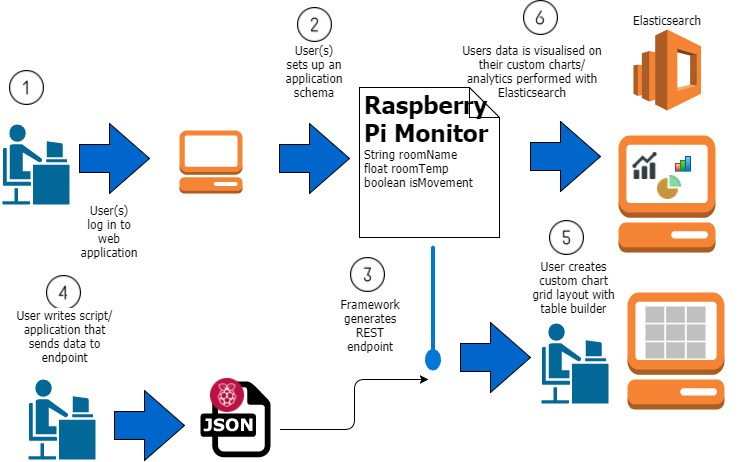
\includegraphics[width=\textwidth,height=\textheight,keepaspectratio]{dynamic_performance_framework_pi_flow}
In this example the user creates a schema in Iris for a raspberry pi. The user has a raspberry pi set up with a sensor to act as a home alarm. The user has written a script on the pi to send JSON data to the schema endpoint in Iris containing room name, room temperature and if there is any movement in the room. Data is being sent every five seconds to Iris. The user then logs into Iris and creates a dashboard for visualising the raspberry pi data.
\end{tcolorbox}
\caption{Raspberry Pi Monitor for Iris}
\end{figure}
\begin{figure}[H]
\begin{tcolorbox}
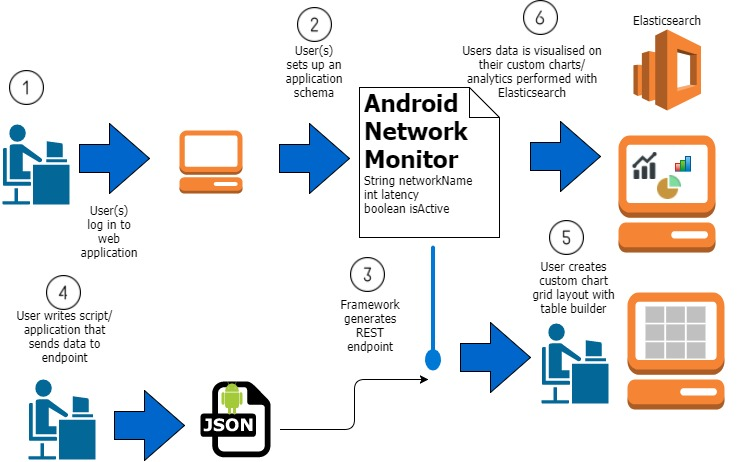
\includegraphics[width=\textwidth,height=\textheight,keepaspectratio]{dynamic_performance_framework_android_flow}
In this example the user creates a schema in Iris for an android application. The android application is sending network data to the Iris generated endpoint, the user sends the network name, latency and if the network is currently active in the form of a JSON object, every five seconds. The user then logs into Iris and build a dashboard to visualise the android data coming into Iris.
\end{tcolorbox}
\caption{Android Network Monitor for Iris}
\end{figure}

\end{document}